
%(BEGIN_QUESTION)
% Copyright 2015, Tony R. Kuphaldt, released under the Creative Commons Attribution License (v 1.0)
% This means you may do almost anything with this work of mine, so long as you give me proper credit

\noindent

\vskip 5pt

\begin{center}
\vskip 5pt 
\textbf{Pådrag -- Nivå 2 }
\vskip 5pt 
\textbf{Arbidsoppdrag på Stasjon 20}
\vskip 5pt 
\textbf{Servomotor}
\end{center}

\textbf{Introduksjon}
I dette arbeidsoppdraget skal du starte opp og styre en servomotor ved hjelp av motion controll blokker. . 


$$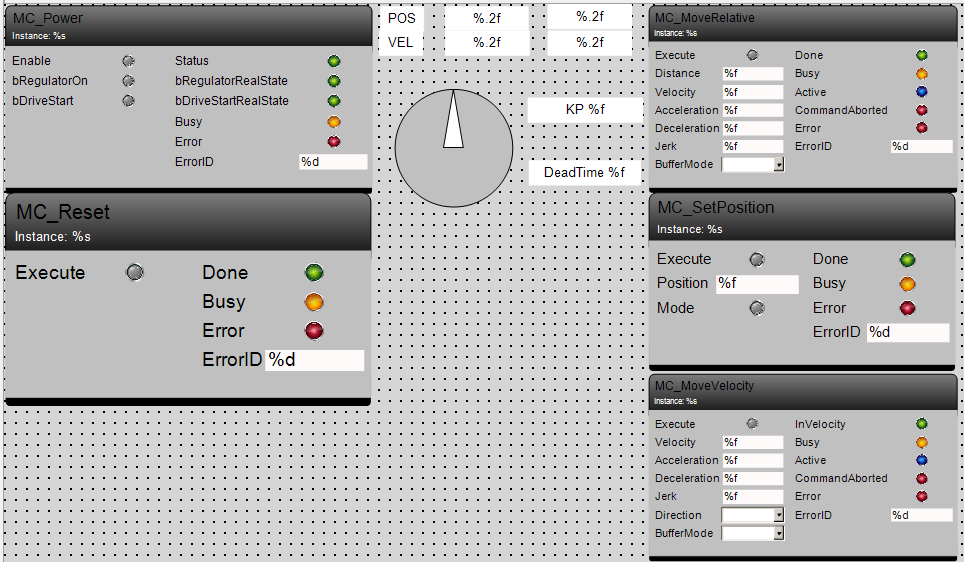
\includegraphics[width=13cm]{i04858x02.png}$$\\
\textbf{Teorioppgaver}\\

\href {https://plcopen.org/system/files/downloads/plcopen_motion_control_part_3_version_2.0.pdf}{Function Blocks for Motion Control}\\


\textbf{Planlegging}

\textbf{Gjennomføring}
\href{https://rfka-my.sharepoint.com/:f:/g/personal/fred-olav_mosdal_skole_rogfk_no/EjCt3CBy6hpFsAqgUV3o8sEBZpsutOKc0eHPvnmOe1rlhg?e=nI1x3c}{Codeys prosjekt}
\textbf{Dokumentasjon}

Beskriv hvordan du planlegger, gjennomfører og dokumenterer denne jobben. 


\vskip 5pt
\begin{center}
\textbf{Arbidsoppdrag}
\vskip 5pt 
\textbf{Programmering av reguleringsstasjon}
\end{center}

\vskip 10pt 
\textbf{Introdusjon}

\vskip 5pt 

\vskip 5pt 

%$$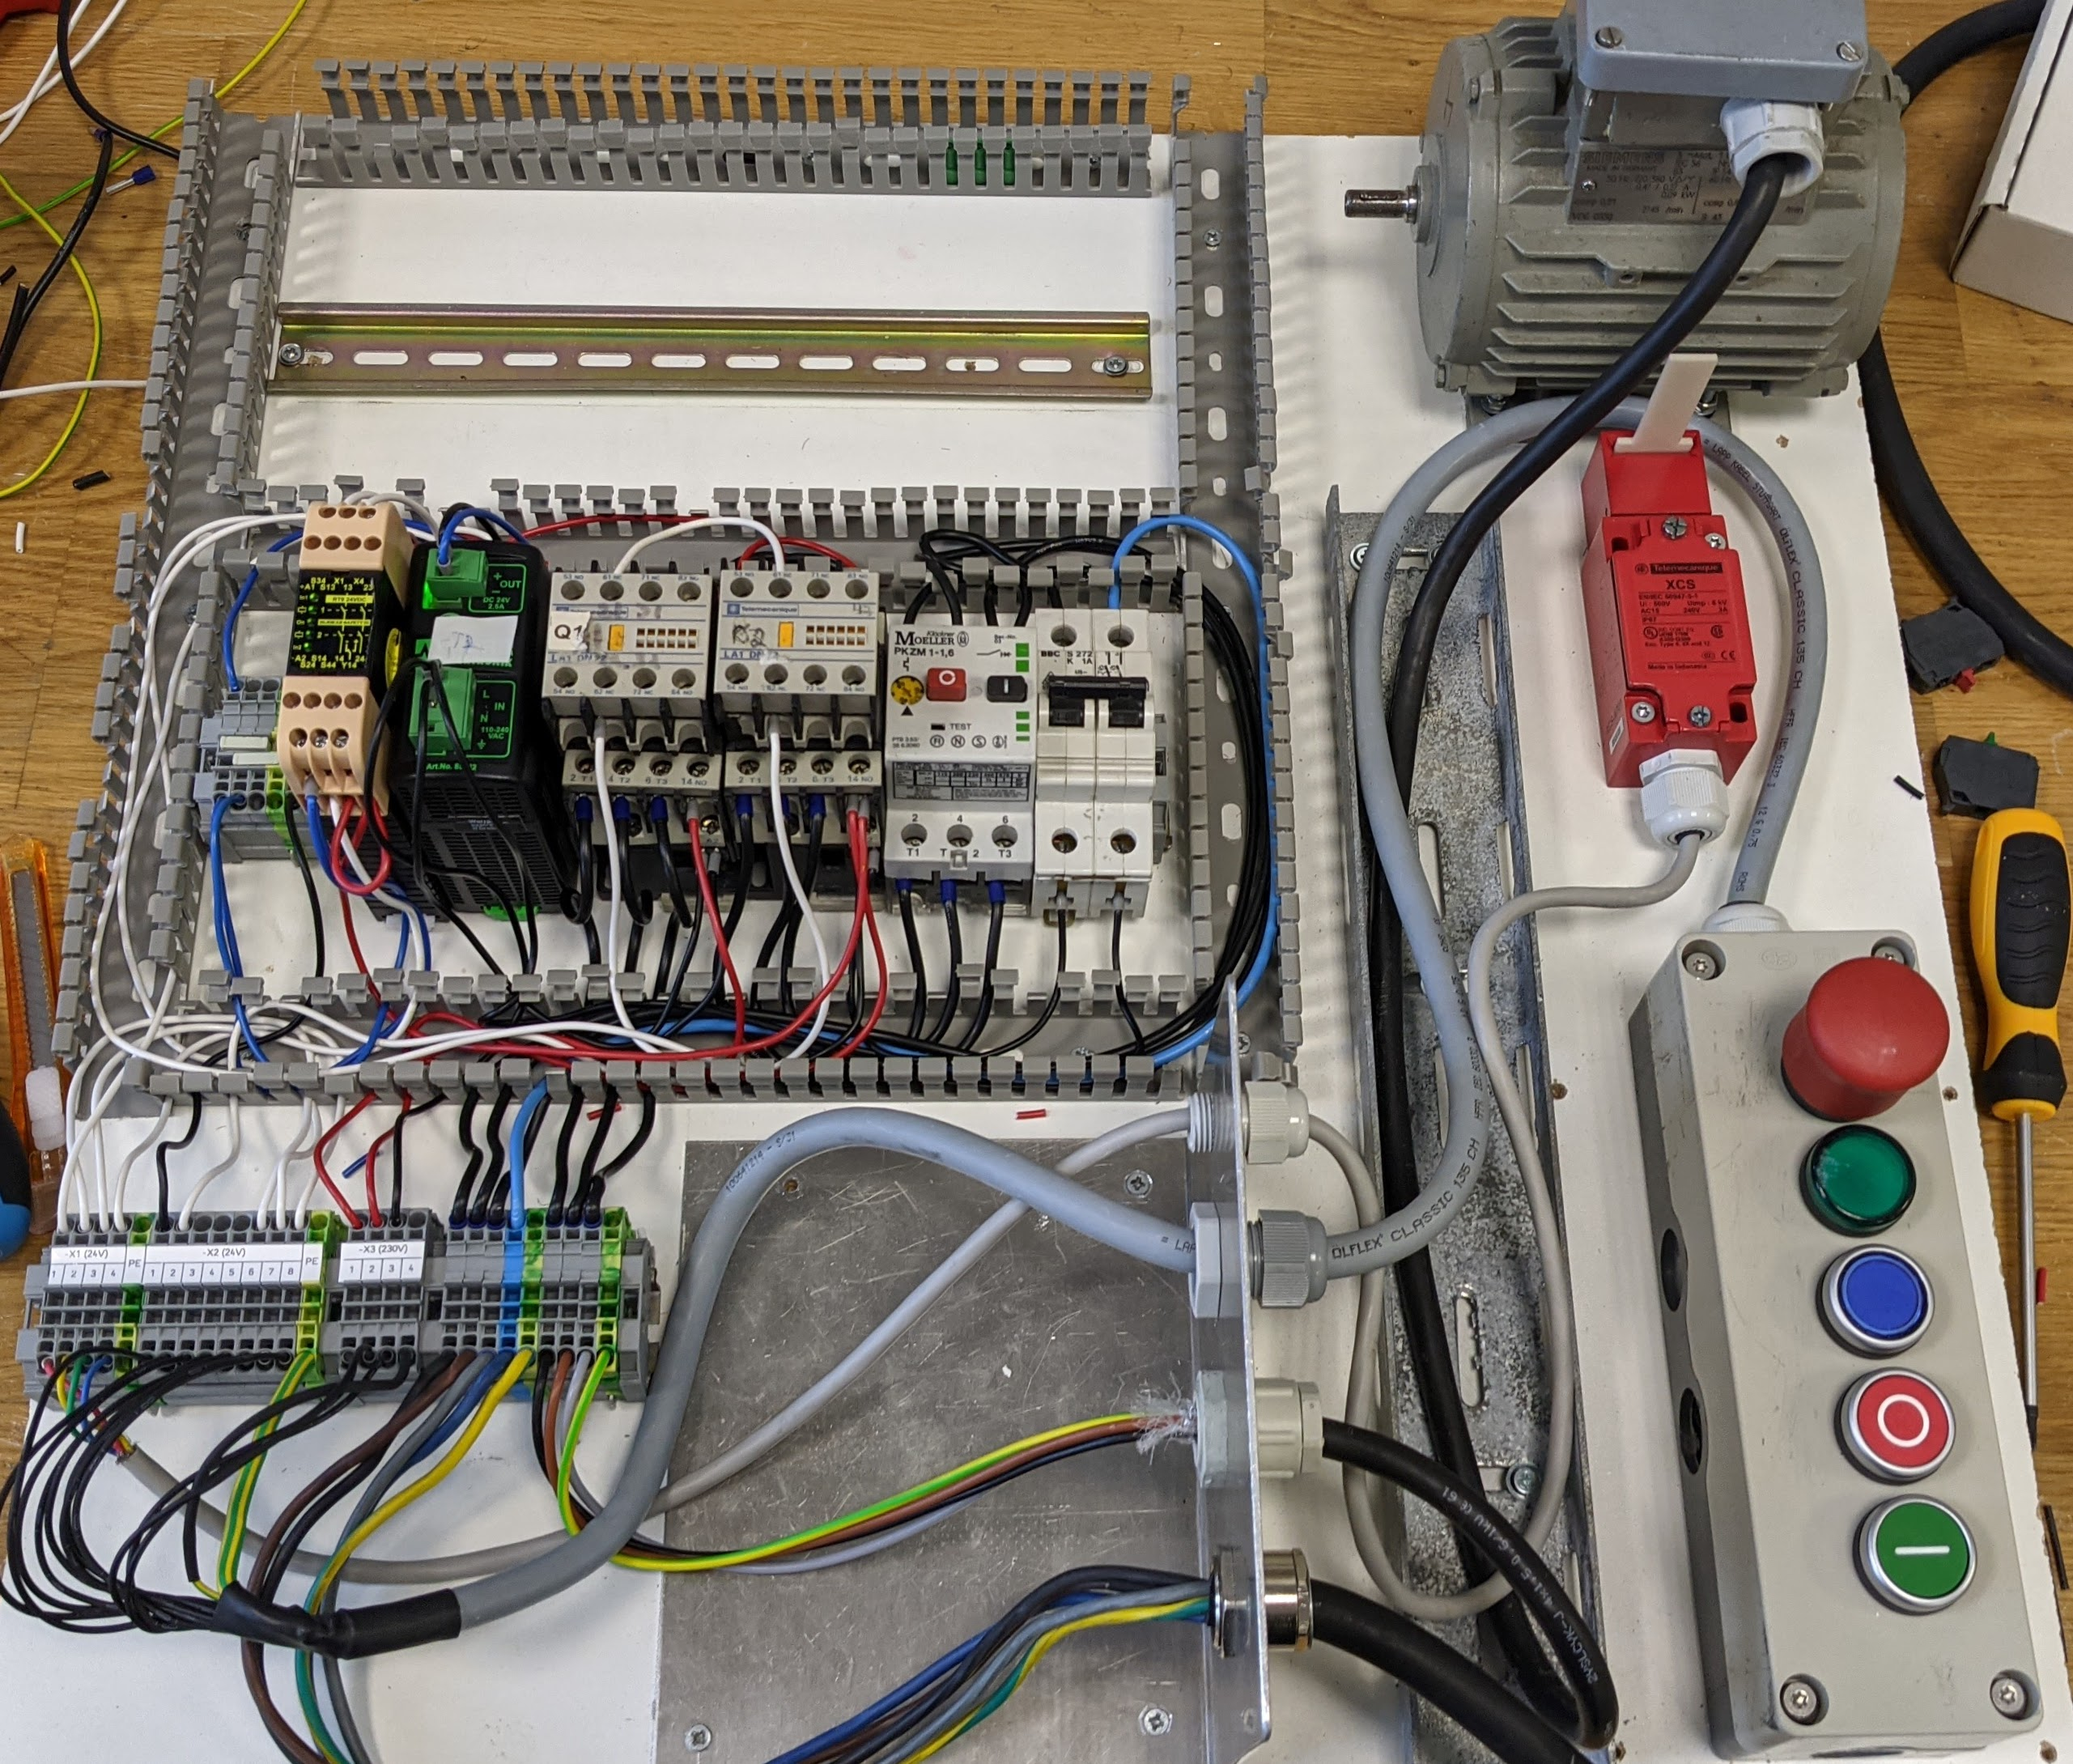
\includegraphics[width=13cm]{i04821x01.jpg}$$\\

\vskip 10pt 
\textbf{Teorioppgaver}

\vskip 5pt 

\vskip 10pt 
\textbf{Planlegging}


\vskip 10pt 
\textbf{Gjennomføring}

\vskip 10pt 
\textbf{Dokumentasjon}

Beskriv hvordan du planlegger, gjennomfører og dokumenterer denne jobben. 



















\underbar{file i04858}
\vfil \eject
%(END_QUESTION)





%(BEGIN_ANSWER)


%(END_ANSWER)





%(BEGIN_NOTES)


%INDEX% Arbeisdoppdrag, Kompetanse, Nivå 1, Stasjonxx, Mal

%(END_NOTES)


